
%%%%%%%%%%%%%%%%%%%%%%%%%%%%%%%%%%%%%%%%%%%%%%%%%%%%%%%%
%
% Copyright (c) 2003-2010 by University of Queensland
% Earth Systems Science Computational Center (ESSCC)
% http://www.uq.edu.au/esscc
%
% Primary Business: Queensland, Australia
% Licensed under the Open Software License version 3.0
% http://www.opensource.org/licenses/osl-3.0.php
%
%%%%%%%%%%%%%%%%%%%%%%%%%%%%%%%%%%%%%%%%%%%%%%%%%%%%%%%%

\section{Steady-state Heat Refraction}
\label{STEADY-STATE HEAT REFRACTION}
Steady-state heat refraction will give us an opportunity to investigate some of the richer features that the \esc package has to offer. One of these is \pycad . The advantage of using \pycad is that it offers an easy method for developing and manipulating complex models. In conjunction with \gmsh we can develop finite element grids that conform to our domain's shape providing accurate modeling of interfaces and boundaries. Another useful function of \pycad is that we can tag specific areas of our domain with labels as we construct them. These labels can then be used in \esc to define properties like material constants and source locations. 

\subsection{Creating the model with \pycad}
\sslist{heatrefraction_mesher001.py and cblib.py}

Our first heat refraction model will be a large anticlinal structure that is experiencing a constant temperature at the surface and a steady heat flux at it's base. Our aim is to show that the temperature flux across the surface is not linear from bottom to top but is in fact warped by the structure of the model and is heavily dependant upon the material properties and shape.

\begin{figure}[h!]
\centerline{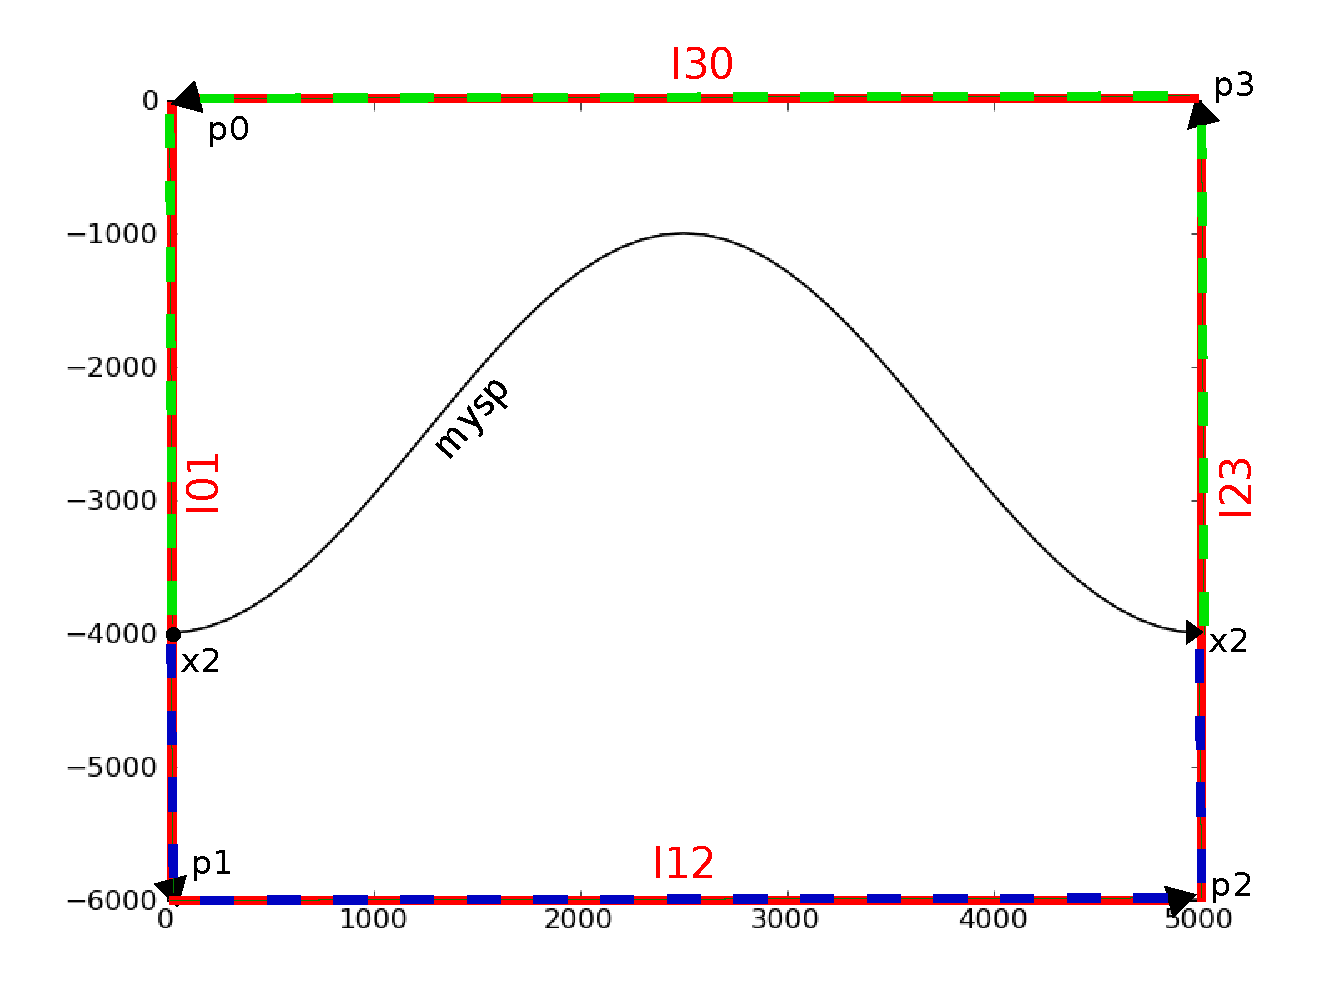
\includegraphics[width=4.in]{figures/anticlineheatrefraction}}
\caption{Heat refraction model with point and line labels.}
\label{fig:anticlinehrmodel}
\end{figure}

We will start by defining our domain and material boundaries using the \pycad module. This example is located in the \esc directory under \exf and a labelled diagram is available in \reffig{fig:anticlinehrmodel}. The dependencies come first and for this example we have:
\begin{python}
from esys.pycad import * #domain constructor
from esys.pycad.gmsh import Design #Finite Element meshing package
from esys.finley import MakeDomain #Converter for escript
import os #file path tool
import numpy as np #numerial python for arrays
from math import * # math package
#used to construct polygons for plotting from pycad
from cblib import getLoopCoords 
\end{python}
There are two modes available in our example. When \verb modal=1  this indicates to the script that we wish to model an anticline. Otherwise when \verb modal=-1  this will model a syncline. The modal operator simply changes the orientation of the boundary function so that it is either upwards or downwards curving. A \verb save_path  has also been defined so that we can easily separate our data from other examples and our scripts. 

It is now possible to start defining our domain and boundaries. There are a few primary constructors in \pycad that build upon each other to define domains and boundaries; the ones we will use are:
\begin{python}
Point() #Create a point in space.
Line() #Creates a line from a number of points.
CurveLoop() #Creates a closed loop from a number of lines.
Surface() #Creates a surface based on a CurveLoop
\end{python}
We start by inputting the variables we need to construct the model.
\begin{python}
#Model Parameters
width=5000.0   #width of model
depth=-6000.0  #depth of model
sspl=51 #number of discrete points in spline
dsp=width/(sspl-1) #dx of spline steps for width
dep_sp=2500.0 #avg depth of spline
h_sp=1500.0 #heigh of spline
orit=-1.0 #orientation of spline 1.0=>up -1.0=>down
\end{python} 
The variables are then used to construct the four corners of our domain, which from the origin has the dimensions of 5000 meters width and -6000 meters depth. This is done with the \verb Point()  function which accepts x, y and z coordinates. Our domain is in two dimensions so z should always be zero. Be careful to define all your constructs in an \textbf{anti-clockwise} manner otherwise the meshing algorithm may fail.
\begin{python}
# Overall Domain
p0=Point(0.0,      0.0, 0.0)
p1=Point(0.0,    depth, 0.0)
p2=Point(width, depth, 0.0)
p3=Point(width,   0.0, 0.0)
\end{python}
Now lines are defined in an \textbf{anti-clockwise} direction using our points. This forms a rectangle around our domain.
\begin{python}
l01=Line(p0, p1)
l12=Line(p1, p2)
l23=Line(p2, p3)
l30=Line(p3, p0)
\end{python}
These lines form the basis for our domain boundary, which is a closed loop.
\begin{python}
c=CurveLoop(l01, l12, l23, l30)
\end{python}
The curve defining our clinal structure is located in approximately the middle of the domain and has a sinusoidal shape. We define the curve by generating points at discrete intervals; 51 in this case, and then create a smooth curve through the points using the \verb Spline()  function.
\begin{python}
# Material Boundary
x=[ Point(i*dsp\
    ,-dep_sp+modal*orit*h_sp*cos(pi*i*dsp/dep_sp+pi))\
     for i in range(0,sspl)\
    ]
mysp = Spline(*tuple(x)) #*tuple() forces x to become a tuple
\end{python}
The start and end points of the spline can be returned to help define the material boundaries.
\begin{python}
x1=Spline.getStartPoint(mysp)
x2=Spline.getEndPoint(mysp)
\end{python}
The top block or material above the clinal/spline boundary is defined in a \textbf{anti-clockwise} manner by creating lines and then a closed loop. As we will be meshing the sub-domain we also need to assign it a planar surface. 
\begin{python}
# TOP BLOCK
tbl1=Line(p0,x1)
tbl2=mysp
tbl3=Line(x2,p3)
tblockloop = CurveLoop(tbl1,tbl2,tbl3,l30)
tblock = PlaneSurface(tblockloop)
\end{python}
It is also necessary to create and export a polygon for \esc so that we can plot the boundaries of our sub-domains. First we take the loop from our block and retrieve its point coordinates with the function \verb getLoopCoords()  and then output it with \modnumpy for our solution script.
\begin{python}
tpg = getLoopCoords(tblockloop)
np.savetxt(os.path.join(save_path,"toppg"),tpg,delimiter=" ")
\end{python}
We must repeat the above for every other sub-domain. In this example there is only one other, the bottom block. The process is fairly similar to the top block but with a few differences. The spline points must be reversed by setting the spline as negative.
\begin{python}
bbl4=-mysp
\end{python}
This reverse spline option unfortunately does not work for the getLoopCoords command, however, the \modmpl polygon tool will accept clock-wise oriented points so we can define a new curve.
\begin{python}
#clockwise check
bblockloop2=CurveLoop(mysp,Line(x2,p2),Line(p2,p1),Line(p1,x1))
bpg = getLoopCoords(bblockloop2)
np.savetxt(os.path.join(save_path,"botpg"),bpg,delimiter=" ")
\end{python}
The last few steps in creating the model take the previously defined domain and sub-domain points and generate a mesh that can be imported into \esc.
To initialise the mesh it first needs some design parameters. In this case we have 2 dimensions \verb dim  and a specified number of finite elements that need to be applied to the domain \verb element_size  . It then becomes a simple task of adding the sub-domains and flux boundaries to the design. Each element of our model can be given an identifier which makes it easier to define the sub-domain properties in the solution script. This is done using the \verb PropertySet()  function. The geometry and mesh are then saved so the \esc domain can be created.
\begin{python}
# Create a Design which can make the mesh
d=Design(dim=2, element_size=200)
# Add the sub-domains and flux boundaries.
d.addItems(PropertySet("top",tblock),PropertySet("bottom",bblock),\
                   PropertySet("linebottom",l12))
# Create the geometry, mesh and \esc domain
d.setScriptFileName(os.path.join(save_path,"heatrefraction_mesh001.geo"))
d.setMeshFileName(os.path.join(save_path,"heatrefraction_mesh001.msh"))
domain=MakeDomain(d, integrationOrder=-1, reducedIntegrationOrder=-1,\
                                   optimizeLabeling=True)
# Create a file that can be read back in to python with mesh=ReadMesh(fileName)
domain.write(os.path.join(save_path,"heatrefraction_mesh001.fly"))
\end{python}
The creation of our domain and its mesh is complete. Now we must create a solution for our steady state problem.

\subsection{Steady-state PDE solution}
\sslist{heatrefraction.py and cblib.py}
While a steady-state solution will not give an indication as to the quantitative heat flow in a model, it is useful because it allows us to visualise the direction of heat transport and the equilibrium state of the model. Also, a steady-state model only requires one iteration to find a solution. We know from \refCh{CHAP HEAT DIFF} that the full form of the heat diffusion PDE can be expressed as follows.
\begin{equation}
\rho c\hackscore p \frac{\partial T}{\partial t} - \kappa \frac{\partial^{2} T}{\partial x^{2}} = q\hackscore H 
\label{eqn:hd2}
\end{equation}
In the steady state PDE however, there is no time dependence. This means that \refEq{eqn:hd2} reduces to
\begin{equation}
- \kappa \frac{\partial^{2} T}{\partial x^{2}} = q\hackscore H 
\label{eqn:sshd}
\end{equation}
where we see our only variables are $\kappa$ the thermal conductivity and the heat source term $q\hackscore H$. Our boundary conditions are similar to earlier problems with some exceptions. Our heat source $q\hackscore H$ is now located at the base of the model and is implemented using our \modpycad identity \textit{linebottom} and we have a constant temperature along the surface of the model where $z=0$. The \modLPDE module's general form as a provision for these cases of the form
\begin{equation}
u=r \textit{    where    } q>0
\label{eqn:bdr}
\end{equation}
using this functionality forces the solution $u$ to equal the value or $r$ wherever the criterion supplied by $q>0$ is true.
The structure of our solution script is similar to those we have used already. We begin by importing the dependencies and defining the PDE and script variables. In this case there are four major variables; \verb qin  is the temperature of our source, \verb Ti  is the temperature on the surface at $z=0$ and our width and depth of the model.
\begin{python}
##ESTABLISHING VARIABLES
qin=70*Milli*W/(m*m) #our heat source temperature is now zero
Ti=290.15*K # Kelvin #the starting temperature of our iron bar
width=5000.0*m
depth=-6000.0*m
\end{python}
The mesh is now imported via the \verb ReadMesh()  function and loaded into a domain variable \verb mymesh . This is followed by the structural polygons. With the mesh imported it is now possible to use our tagging property to set up our PDE coefficients. In this case $\kappa$ is set via the \verb setTaggedValue()  function which takes two arguments, the name of the tagged points and the value to assign to them. 
\begin{python}
mymesh=ReadMesh(os.path.join(saved_path,"heatrefraction_mesh001.fly"))
tpg = np.loadtxt(os.path.join(saved_path,"toppg"))
tpgx = tpg[:,0]
tpgy = tpg[:,1]
bpg = np.loadtxt(os.path.join(saved_path,"botpg"))
bpgx = bpg[:,0]
bpgy = bpg[:,1]

# set up kappa (thermal conductivity across domain) using tags
kappa=Scalar(0,Function(mymesh))
kappa.setTaggedValue("top",2.0)
kappa.setTaggedValue("bottom",4.0)
\end{python}
Setting up the PDE is a little more complicated. The linear PDE \verb mypde  is again assigned the domain \verb mymesh  and \verb A  is set. \verb qH  is set on the boundary by creating \verb qH  as a function space of type \verb FunctionOnBoundary  which is in turn based on \verb mymesh  . We can then set the tagged value \textit{linebottom} to the condition \verb qin  . We also need to use our condition from \refEq{eqn:bdr}. By extracting \verb x  we can set the domain at zero to 1 and everywhere else 0 via the \verb whereZero()  function. This is put into \verb q  and \verb r  is set to \verb Ti  our temperature at the surface. Note \verb y=qH  . As there is no time derivative in the equation we do not have any iterative steps and there is one solution to the problem. This is found in the step \verb T=mypde.getSolution()  .
\begin{python}
#... generate functionspace...
#... open PDE ...
mypde=LinearPDE(mymesh)
#define first coefficient
mypde.setValue(A=kappa*kronecker(mymesh))

# ... set initial temperature ....
x=mymesh.getX()

qH=Scalar(0,FunctionOnBoundary(mymesh))
qH.setTaggedValue("linebottom",qin)
mypde.setValue(q=whereZero(x[1]),r=Ti)
mypde.setValue(y=qH)

# get steady state solution.
T=mypde.getSolution()
\end{python}
The problem is now solved and plotting is required to visualise the data.

\subsection{Line profiles of 2D data}
It is possible to take slices or profile sections of 2d data using \mpl. To achieve this there are three major steps, firstly the solution must be smoothed across the domain using the \verb projector()  function.
\begin{python}
proj=Projector(mymesh)
smthT=proj(T)
\end{python}
The data must then be moved to a regular grid.
\begin{python}
xi,yi,zi = toRegGrid(smthT,mymesh,200,200,width,depth)
\end{python}
The profile can then be plotted by taking a slice of the data output \verb zi  . 
\begin{python}
cut=int(len(xi)/2)
pl.clf()
pl.plot(zi[:,cut],yi)
pl.title("Heat Refraction Temperature Depth Profile")
pl.xlabel("Temperature (K)")
pl.ylabel("Depth (m)")
\end{python}
This process can be repeated for various variations of the solution. In this case we have temperature, temperature gradient, thermal conductivity and heat flow \reffig{figs:dps}.
\begin{figure}
\centering
    \subfigure[Temperature Depth Profile]{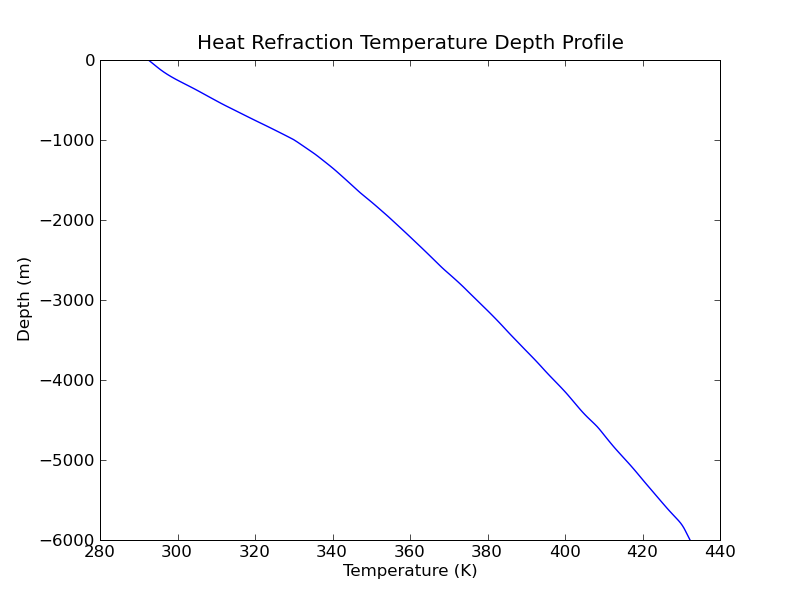
\includegraphics[width=3in]{figures/heatrefraction001tdp.png}\label{fig:tdp}}
    \subfigure[Temperature Gradient Depth Profile]{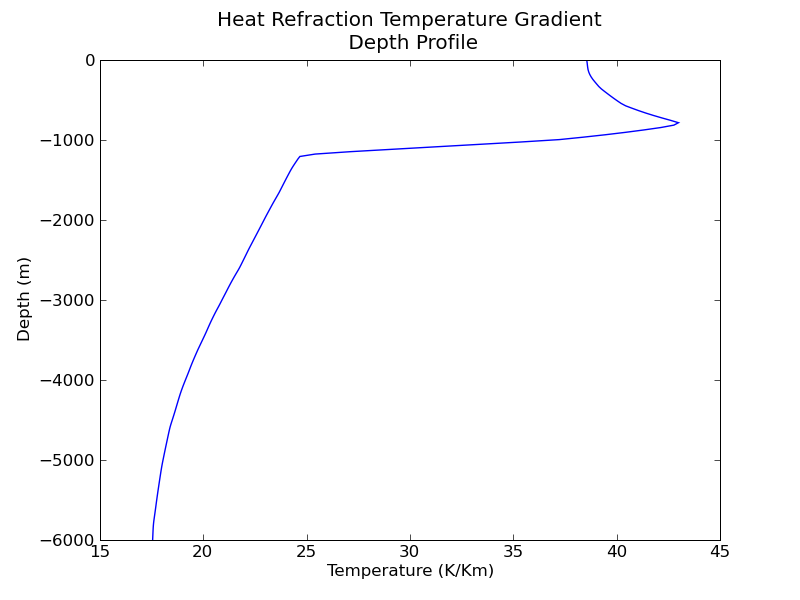
\includegraphics[width=3in]{figures/heatrefraction001tgdp.png}\label{fig:tgdp}}
    \subfigure[Thermal Conductivity Profile]{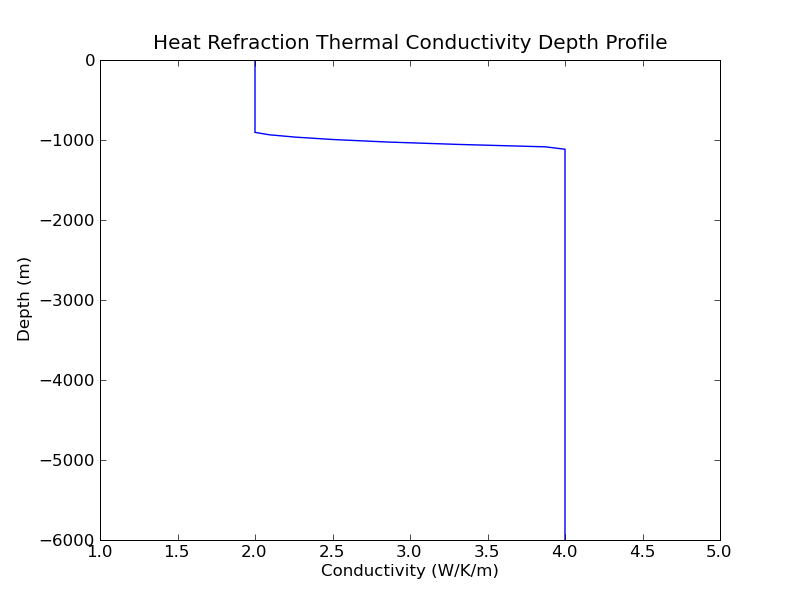
\includegraphics[width=3in]{figures/heatrefraction001tcdp.png}\label{fig:tcdp}}
    \subfigure[Heat Flow Depth Profile]{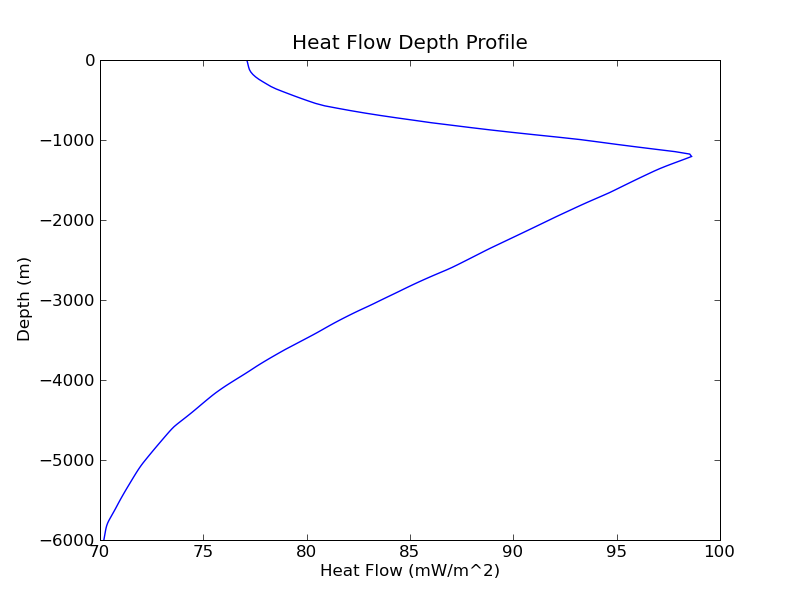
\includegraphics[width=3in]{figures/heatrefraction001hf.png}\label{fig:hf}}
  \caption{Depth profiles down centre of model.}
  \label{figs:dps}
\end{figure}




\subsection{Quiver plots in \mpl}
To visualise this data we are going to do three things. Firstly we will generate the gradient of the solution and create some quivers or arrows that describe the gradient. Then we need to generate some temperature contours and thirdly, we will create some polygons from our meshing output files to show our material boundaries.

The first step is very easily provided by \esc, where we can use the \verb grad()  function to generate our gradient. It is then necessary to mould the solution to the domain node points. We do this by first extracting the nodes to \verb oldspacecoords  and transforming them via interpolation to suit our solution which is in the function space form of \verb T  .
\begin{python}
# calculate gradient of solution for quiver plot
qu=-kappa*grad(T)

# rearrange mymesh to suit solution function space      
oldspacecoords=mymesh.getX()
coords=Data(oldspacecoords, T.getFunctionSpace())
\end{python}
Now the number of quivers we want is specified as $20 \times 20 = 400$ and their locations calculated based on our coordinates in \verb qu  . All our data is then transformed to tuples for \modmpl .
\begin{python}
quivshape = [20,20] #quivers x and quivers y
# function to calculate quiver locations
qu,qulocs = toQuivLocs(quivshape,width,depth,qu)

kappaT = kappa.toListOfTuples(scalarastuple=False)
coordsK = Data(oldspacecoords, kappa.getFunctionSpace())
coordKX, coordKY = toXYTuple(coordsK)
      
tempT = T.toListOfTuples(scalarastuple=False)
coordX, coordY = toXYTuple(coords)
\end{python}
In a similar fashion to the contouring, our data needs to be transferred to a regular grid to contour the temperature. Our polygons are handled by the \verb fill()  function making sure they are ordered to the lowest level of the plot beneath all other data. Labelling is then added and finally the Quivers using the \verb quiver()  function. More detail on each \modmpl function is available from the \modmpl website.
\begin{python}
xi = np.linspace(0.0,width,100)
yi = np.linspace(depth,0.0,100)
# grid the data.
zi = pl.matplotlib.mlab.griddata(coordX,coordY,tempT,xi,yi)
ziK = pl.matplotlib.mlab.griddata(coordKX,coordKY,kappaT,xi,yi)
# contour the gridded data, plotting dots at the randomly spaced data points.
pl.matplotlib.pyplot.autumn()

CKL = pl.fill(tpgx,tpgy,'brown',bpgx,bpgy,'red',zorder=-1000)
#~ CK = pl.contourf(xi,yi,ziK,2)
CS = pl.contour(xi,yi,zi,5,linewidths=0.5,colors='k')

pl.clabel(CS, inline=1, fontsize=8)
pl.title("Heat Refraction across a clinal structure.")
pl.xlabel("Horizontal Displacement (m)")
pl.ylabel("Depth (m)")
#~ CB = pl.colorbar(CS, shrink=0.8, extend='both')
pl.savefig(os.path.join(saved_path,"heatrefraction001_cont.png"))

QUIV=pl.quiver(qulocs[:,0],qulocs[:,1],qu[:,0],qu[:,1],angles='xy',color="white")
pl.title("Heat Refraction across a clinal structure \n with gradient quivers.")
pl.savefig(os.path.join(saved_path,"heatrefraction001_contqu.png"))
\end{python} 
The data has now been plotted.
\begin{figure}[ht]
\centerline{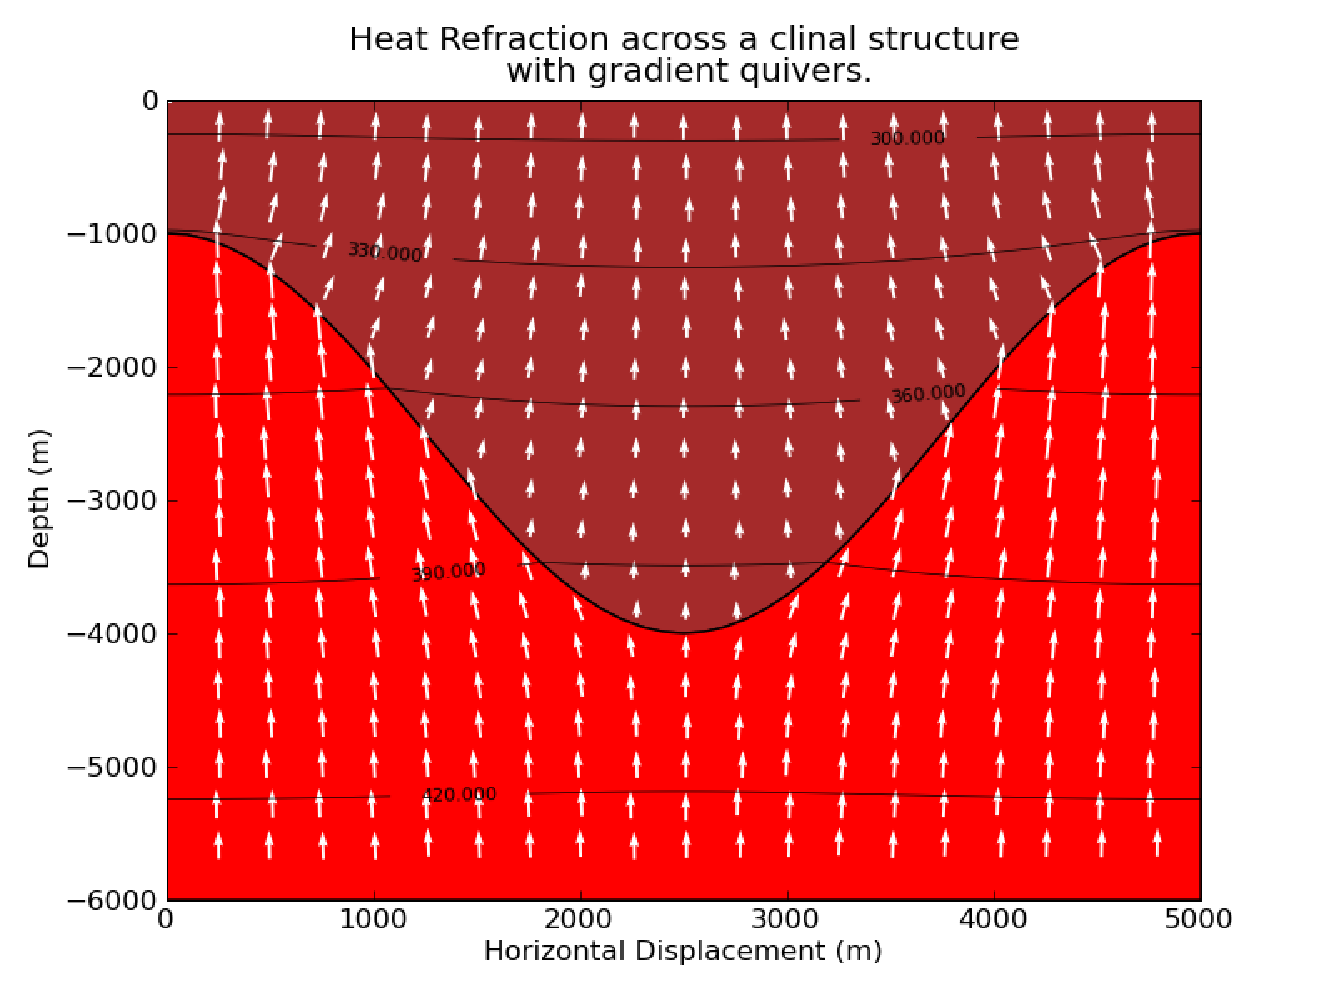
\includegraphics[width=4.in]{figures/heatrefraction001contqu}}
\caption{Heat refraction model with gradient indicated by quivers.}
\label{fig:hr001qumodel}
\end{figure}

\newpage
\subsection{Fault and Overburden Model}
A slightly more complicated model can be found in the examples \textit{heatrefraction_mesher002.py} and \textit{heatrefractoin002.py} where three blocks are used within the model.
\begin{figure}[ht]
\centerline{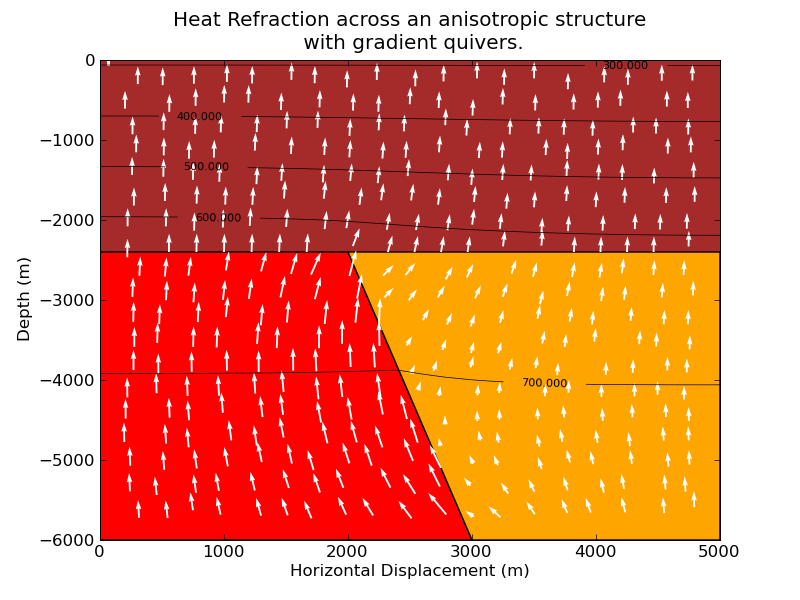
\includegraphics[width=4.in]{figures/heatrefraction002contqu}}
\caption{Heat refraction model with three blocks and gradient quivers.}
\end{figure}

